% Created 2010-06-02 Wed 22:46
\documentclass[11pt,a4paper]{report}
\usepackage[utf8]{inputenc}
\usepackage[spanish]{babel}
\usepackage{times}
\usepackage{amsmath}
\usepackage{amstext}
\usepackage{lscape}
\usepackage{color}
\setlength{\parindent}{7mm} %sangria la primera linea
\usepackage[pdftex=true,colorlinks=true,plainpages=false]{hyperref} % Soporte hipertexto

%PROFUNDIDAD DE LA TABLA DE CONTENIDO O ÍNDICE GENERAL
\setcounter{tocdepth}{4}
\setcounter{secnumdepth}{3}

\usepackage{graphicx}
\sloppy % suaviza las reglas de ruptura de líneas de LaTeX

\title{Stickmotion}
\author{grupo}
\date{Córdoba, 3 de Junio de 2010}

\begin{document}

\maketitle

\setcounter{tocdepth}{3}
\tableofcontents
\vspace*{1cm}





\chapter{Diseño de la arquitectura lógica, diagrama de paquetes.}
\label{sec-1}


En este capítulo se agruparán las clases mediante el empleo de paquetes que se organizarán mostrando sus relaciones de importación/exportación en un diagrama de paquetes. \\

Los diagramas de paquetes se usan para representar relaciones
lógicas entre distintos elementos como pueden ser clases y casos de
usos, que mantienen una relación semántica entre ellos. \\

\section{Identificación de paquetes}
\label{sec-1.1}


\begin{figure}[htb]
\centerline{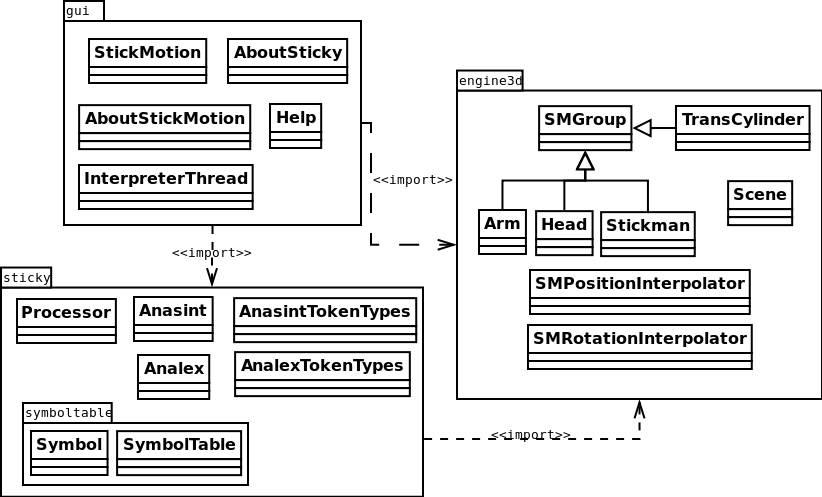
\includegraphics[width=\textwidth]{imagenes/paquetes.png}}
\caption{\label{fig:dpaquetes}Diagrama de paquetes de la aplicación}
\end{figure}


Se empaquetarán las clases agrupándolas en los siguientes paquetes, correspondiendose con los componentes funcionales en los que se descompuso el sistema en el análisis de requisitos. \\

En la figura \ref{fig:dpaquetes} se muestra el diagrama indicando las relaciones de importación que se realizan entre los distintos paquetes. \\


\begin{itemize}
\item \textbf{Paquete engine3D (Motor 3D de animaciones).} Incluyendo las clases:

\begin{itemize}
\item SMGroup
\item TransCylinder
\item Arm
\item Head
\item Stickman
\item Scene
\item SMPositionInterpolator
\item SMRotationInterpolator
\end{itemize}

\item \textbf{Paquete ``gui'' (Interfaz gráfica y editor).} Incluyendo las clases:

\begin{itemize}
\item StickMotion
\item AboutSticky
\item AboutStickMotion
\item Help
\item InterpreterThread
\end{itemize}

\item \textbf{Paquete ``sticky'' (Procesador del lenguaje Sticky).} Incluyendo las clases:

\begin{itemize}
\item Processor
\item Anasint
\item Analex
\item AnasintTokenTypes
\item AnalexTokenTypes
\end{itemize}

\item \textbf{Subpaquete ``tablasimbolos''.} Contenido en el paquete sticky, incluye las clases:

\begin{itemize}
\item Symbol
\item SymbolTable
\end{itemize}

\end{itemize}

\end{document}